
\documentclass[11pt,a4paper]{article}
\usepackage{ucs}
\usepackage[utf8x]{inputenc}
\usepackage[T1]{fontenc}
\usepackage{ngerman}
\usepackage{amsmath,amssymb,amstext}
\usepackage{tikz}
\title{Rechnerstrukturen Blatt 3}
\author{Sven Marquardt}
\date{\today}
\input{kvmacros}
\usetikzlibrary{automata}
\usetikzlibrary{positioning}
\usetikzlibrary{topaths}
\begin{document}
Aufgabe3.1\\
Die Schaltung soll einen Zähler darstellen der in 3er Schritten vorwärts oder rückwärts Zählt. Das Umstellen der Zählrichtung erfolgt durch den Schalter $x_0$.\\
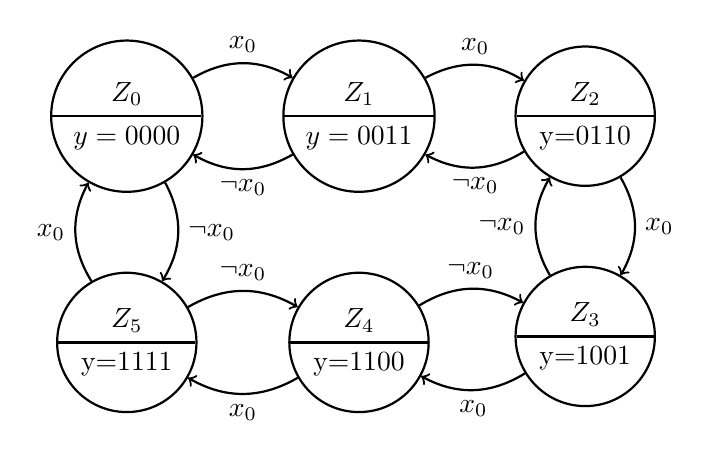
\begin{tikzpicture}[auto,thick]
	\node[state with output] (Z0) {$Z_0$ \nodepart {lower} $y=0000$};
	\node[state with output, right=of Z0] (Z1) {$Z_1$ \nodepart {lower} $y=0011$};
	\node[state with output, right=of Z1] (Z2) {$Z_2$ \nodepart {lower} y=0110};
	\node[state with output, below=of Z2] (Z3) {$Z_3$ \nodepart {lower} y=1001};
	\node[state with output, below=of Z1] (Z4) {$Z_4$ \nodepart {lower} y=1100};
	\node[state with output, below=of Z0] (Z5) {$Z_5$ \nodepart {lower} y=1111};
	\path[->] (Z0)	edge [bend left]		node	{$x_0$}(Z1)
			  		edge [bend left]		node[right]	{$\neg x_0$}(Z5)
			  (Z1)	edge [bend left]		node	{$\neg x_0$}(Z0)
			  		edge [bend left]		node	{$x_0$}(Z2)
			  (Z2)	edge [bend left]		node	{$\neg x_0$}(Z1)
			  		edge [bend left]		node	{$x_0$}(Z3)
			  (Z3)	edge [bend left]		node	{$\neg x_0$}(Z2)
			  		edge [bend left]		node	{$x_0$}(Z4)
			  (Z4)	edge [bend left]		node	{$\neg x_0$}(Z3)
			  		edge [bend left]		node	{$x_0$}(Z5)
			  (Z5)	edge [bend left]		node[left]	{$x_0$}(Z0)			  		
			  		edge [bend left]		node	{$\neg x_0$}(Z4);
\end{tikzpicture}
\\
A=$ ( X,Y,Z, \delta, \mu ) $ ,mit\\
$X= \lbrace 0,1 \rbrace$\\
$Y= \lbrace 0000,0011,0110,1001,1100,1111 \rbrace$\\
$Z= \lbrace 000,001,010,011,100,101 \rbrace$\\
$\delta : Z \times X \rightarrow Z$\\
$\mu : Z \rightarrow Y$\\ \\
Dazu die Wertetabelle \\ \\
\begin{tabular}{c | c | c | c | c | | c | c | c | c | | c | c | c | c}
$x_0$&Z&$z_2$&$z_1$&$z_0$&$y_3$&$y_2$&$y_1$&$y_0$&$Z^+$&$z^+_2$&$z^+_1$&$z^+_0$ \\ \hline
0&$Z_0$&0&0&0&0&0&0&0&$Z_1$&0&0&1\\
0&$Z_1$&0&0&1&0&0&1&1&$Z_2$&0&1&0\\
0&$Z_2$&0&1&0&0&1&1&0&$Z_3$&0&1&1\\
0&$Z_3$&0&1&1&1&0&0&1&$Z_4$&1&0&0\\
0&$Z_4$&1&0&0&1&1&0&0&$Z_5$&1&0&1\\
0&$Z_5$&1&0&1&1&1&1&1&$Z_0$&0&0&0\\
0&--&1&1&0&*&*&*&*&--&*&*&*\\
0&--&1&1&1&*&*&*&*&--&*&*&*\\ \hline
1&$Z_0$&0&0&0&0&0&0&0&$Z_5$&1&0&1\\
1&$Z_1$&0&0&1&0&0&1&1&$Z_0$&0&0&0\\
1&$Z_2$&0&1&0&0&1&1&0&$Z_1$&0&0&1\\
1&$Z_3$&0&1&1&1&0&0&1&$Z_2$&0&1&0\\
1&$Z_4$&1&0&0&1&1&0&0&$Z_3$&0&1&1\\
1&$Z_5$&1&0&1&1&1&1&1&$Z_4$&1&0&0\\
1&--&1&1&0&*&*&*&*&--&*&*&*\\
1&--&1&1&1&*&*&*&*&--&*&*&*\\
\end{tabular}\\
\\ \\  \\
Daraus ergeben sich folgende KV-Diagramme für $z^+_2,z^+_1$ und $z^+_0$.\\
$z^+_2$
\karnaughmap{4}{}{{$x_0$}{$z_2$}{$z_1$}{$z_0$}}{000110**100001**}{}
$z^+_1$
\karnaughmap{4}{}{{$x_0$}{$z_2$}{$z_1$}{$z_0$}}{011000**000101}{}\\
$z^+_0$
\karnaughmap{4}{}{{$x_0$}{$z_2$}{$z_1$}{$z_0$}}{101010**101010**}{}\\ \\ \\ \\
Folglich bilden folgende KV-Diagramme die Minimierung der Ausgangsfunktion.\\
$y_3$
\karnaughmap{3}{}{{$z_2$}{$z_1$}{$z_0$}}{000111**}{}
$y_2$
\karnaughmap{3}{}{{$z_2$}{$z_1$}{$z_0$}}{001011**}{}\\
$y_1$
\karnaughmap{3}{}{{$z_2$}{$z_1$}{$z_0$}}{011001**}{}
$y_0$
\karnaughmap{3}{}{{$z_2$}{$z_1$}{$z_0$}}{010101**}{}\\ \\ \\

Aufgabe 3.2\\
In dieser Aufgabe soll eine Ampel implementiert werden die Automatisch läuft. Heißt nach einer gewissen Zeit gibt es Automatisch grün für die Fußgänger, ohne dass ein Knopf gedrückt werden muss. Es ist also ein autonomer Automat. Folglich beschreibt folgender Automat die Funktion der Ampel. \\
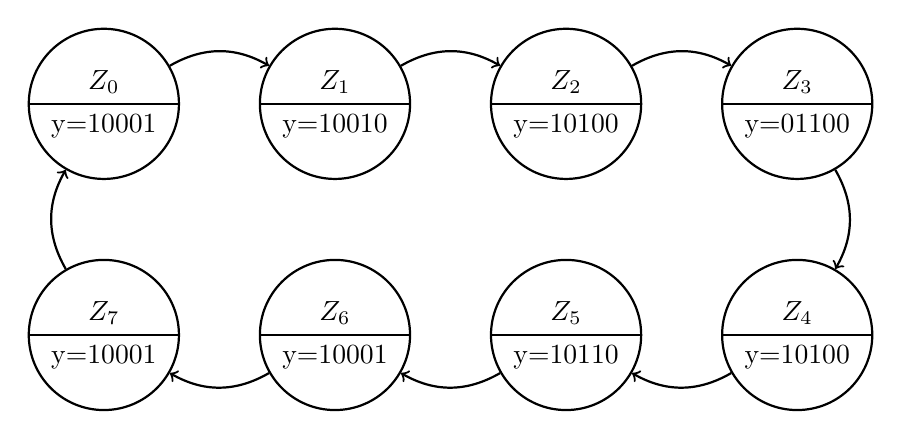
\begin{tikzpicture}[auto,thick]
	\node[state with output] (Z0) {$Z_0$ \nodepart {lower} y=10001};
	\node[state with output, right=of Z0] (Z1) {$Z_1$ \nodepart {lower} y=10010};
	\node[state with output, right=of Z1] (Z2) {$Z_2$ \nodepart {lower} y=10100};
	\node[state with output, right=of Z2] (Z3) {$Z_3$ \nodepart {lower} y=01100};
	\node[state with output, below=of Z3] (Z4) {$Z_4$ \nodepart {lower} y=10100};
	\node[state with output, below=of Z2] (Z5) {$Z_5$ \nodepart {lower} y=10110};
	\node[state with output, below=of Z1] (Z6) {$Z_6$ \nodepart {lower} y=10001};
	\node[state with output, below=of Z0] (Z7) {$Z_7$ \nodepart {lower} y=10001};
	\path[->]
	(Z0)	edge [bend left]	node{}	(Z1)
	(Z1)	edge [bend left]	node{}	(Z2)
	(Z2)	edge [bend left]	node{}	(Z3)
	(Z3)	edge [bend left]	node{}	(Z4)
	(Z4)	edge [bend left]	node{}	(Z5)
	(Z5)	edge [bend left]	node{}	(Z6)
	(Z6)	edge [bend left]	node{}	(Z7)
	(Z7)	edge [bend left]	node{}	(Z0);
\end{tikzpicture}\\ \\
$A= (Y,Z,\delta,\mu)$ , mit\\
$Y= \lbrace 10001,10010,10100,01100,10110 \rbrace$ \\
$Z=\lbrace 000,001,010,011,100,101,110,111 \rbrace$ \\
$\delta : Z \rightarrow Z$\\
$\mu : Z \rightarrow Y$\\
\begin{tabular}{ c | c | c | c | | c | c | c | | c | c | c | c | c | c | | c | c | c | c | c}
Z&$z_2$&$z_1$&$z_0$&$z^+_2$&$z^+_1$&$z^+_0$&$J_2$&$K_2$&$J_1$&$K_1$&$J_0$&$K_0$&$y_4$&$y_3$&$y_2$&$y_1$&$y_0$ \\ \hline
$Z_0$&0&0&0&0&0&1&0&*&0&*&1&*&1&0&0&0&1\\
$Z_1$&0&0&1&0&1&0&0&*&1&*&*&1&1&0&0&1&0\\
$Z_2$&0&1&0&0&1&1&0&*&*&0&1&*&1&0&1&0&0\\
$Z_3$&0&1&1&1&0&0&1&*&*&1&*&1&0&1&1&0&0\\
$Z_4$&1&0&0&1&0&1&*&0&0&*&1&*&1&0&1&0&0\\
$Z_5$&1&0&1&1&1&0&*&0&1&*&*&1&1&0&1&1&0\\
$Z_6$&1&1&0&1&1&1&*&0&*&0&1&*&1&0&0&0&1\\
$Z_7$&1&1&1&0&0&0&*&1&*&1&*&1&1&0&0&0&1\\ \hline
\end{tabular}\\ \\
Die Minimierung der Zustandsübergangsfunktion \\
$J_2$ 
\karnaughmap{3}{}{{$z_2$}{$z_1$}{$z_0$}}{0001****}{} $K_2$
\karnaughmap{3}{}{{$z_2$}{$z_1$}{$z_0$}}{****0001}{}\\
$J_1$
\karnaughmap{3}{}{{$z_2$}{$z_1$}{$z_0$}}{01**01**}{}
$K_1$
\karnaughmap{3}{}{{$z_2$}{$z_1$}{$z_0$}}{**01**01}{}\\
$J_0$
\karnaughmap{3}{}{{$z_2$}{$z_1$}{$z_0$}}{1*1*1*1*}{}
$K_0$
\karnaughmap{3}{}{{$z_2$}{$z_1$}{$z_0$}}{*1*1*1*1}{}\\ \\
$y_4$
\karnaughmap{3}{}{{$z_2$}{$z_1$}{$z_0$}}{11110111}{}
$y_3$
\karnaughmap{3}{}{{$z_2$}{$z_1$}{$z_0$}}{00001000}{}\\
$y_2$
\karnaughmap{3}{}{{$z_2$}{$z_1$}{$z_0$}}{00011110}{}
$y_1$
\karnaughmap{3}{}{{$z_2$}{$z_1$}{$z_0$}}{00100010}{}\\
$y_0$
\karnaughmap{3}{}{{$z_2$}{$z_1$}{$z_0$}}{11000001}{}\\

Aufgabe 3.3\\
In dieser Aufgabe soll die Ampelschaltung von 3.2 erweitert werden um einen  Bedarfsknopf. Die Ampel der Fußgänger soll nun nur grün zeigen, wenn zuvor ein Taster betätigt wurde. Ohne betätigen des Tasters bleibt  der Zustand der Ampel für die Fußgänger auf rot und für die Autofahrer auf grün. Folgender Automat beschreibt die Ampel.\\ 
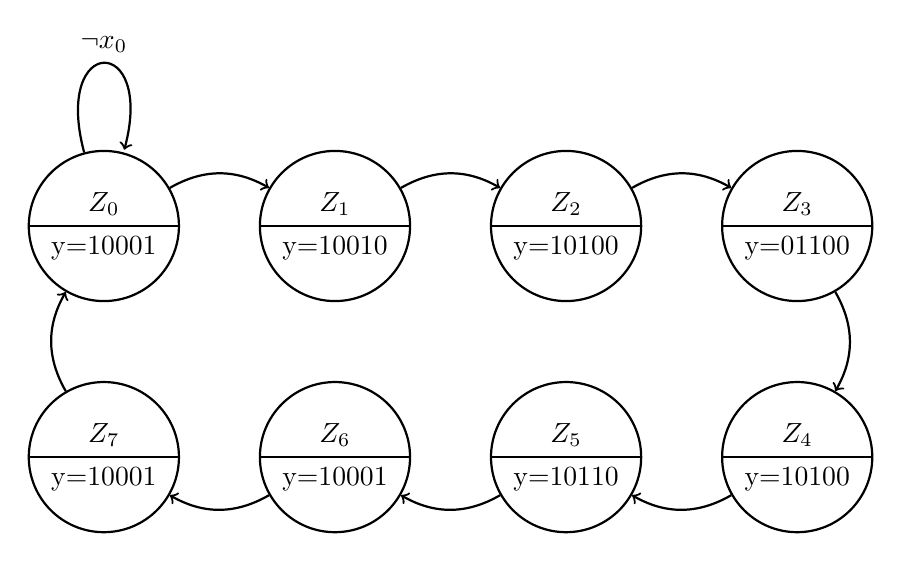
\begin{tikzpicture}[auto,thick]
	\node[state with output] (Z0) {$Z_0$ \nodepart {lower} y=10001};
	\node[state with output, right=of Z0] (Z1) {$Z_1$ \nodepart {lower} y=10010};
	\node[state with output, right=of Z1] (Z2) {$Z_2$ \nodepart {lower} y=10100};
	\node[state with output, right=of Z2] (Z3) {$Z_3$ \nodepart {lower} y=01100};
	\node[state with output, below=of Z3] (Z4) {$Z_4$ \nodepart {lower} y=10100};
	\node[state with output, below=of Z2] (Z5) {$Z_5$ \nodepart {lower} y=10110};
	\node[state with output, below=of Z1] (Z6) {$Z_6$ \nodepart {lower} y=10001};
	\node[state with output, below=of Z0] (Z7) {$Z_7$ \nodepart {lower} y=10001};
	\path[->]
	(Z0)	edge [bend left]	node{}	(Z1)
	(Z0)	edge [loop above]			node[swap]{$\neg x_0$}	()
	(Z1)	edge [bend left]	node{}	(Z2)
	(Z2)	edge [bend left]	node{}	(Z3)
	(Z3)	edge [bend left]	node{}	(Z4)
	(Z4)	edge [bend left]	node{}	(Z5)
	(Z5)	edge [bend left]	node{}	(Z6)
	(Z6)	edge [bend left]	node{}	(Z7)
	(Z7)	edge [bend left]	node{}	(Z0);
\end{tikzpicture}\\ \\ 
$A=(X,Y,Z, \delta, \mu )$, mit\\
$X=\lbrace 0,1 \rbrace$\\
$Y= \lbrace 10001,10010,1010,01100,10100 \rbrace$\\
$Z=\lbrace 000,001,010,011,100,101,110,111 \rbrace$ \\
$\delta : Z \times X \rightarrow Z$\\
$\mu : Z \rightarrow Y$\\ \\
Die Wertetabelle dazu\\
\begin{tabular}{c | c | c | c | c | | c | c | c | | c | c | c | c | c | c | | c | c | c | c | c}
$x_0$&Z&$z_2$&$z_1$&$z_0$&$z^+_2$&$z^+_1$&$z^+_0$&$J_2$&$K_2$&$J_1$&$K_1$&$J_0$&$K_0$&$y_4$&$y_3$&$y_2$&$y_1$&$y_0$ \\ \hline
0&$Z_0$&0&0&0&0&0&0&0&*&0&*&0&*&1&0&0&0&1\\
0&$Z_1$&0&0&1&0&1&0&0&*&1&*&*&1&1&0&0&0&1\\
0&$Z_2$&0&1&0&0&1&1&0&*&*&0&1&*&1&0&0&0&1\\
0&$Z_3$&0&1&1&1&0&0&1&*&*&1&*&1&1&0&0&0&1\\
0&$Z_4$&1&0&0&1&0&1&*&0&0&*&1&*&1&0&0&0&1\\
0&$Z_5$&1&0&1&1&1&0&*&0&1&*&*&1&1&0&0&1&1\\
0&$Z_6$&1&1&0&1&1&1&*&0&*&0&1&*&1&0&0&0&1\\
0&$Z_7$&1&1&1&0&0&0&*&1&*&1&*&1&1&0&0&0&1\\ \hline
1&$Z_0$&0&0&0&0&0&1&0&*&0&*&1&*&1&0&0&0&1\\
1&$Z_1$&0&0&1&0&1&0&0&*&1&*&*&1&1&0&0&1&0\\
1&$Z_2$&0&1&0&0&1&1&0&*&*&0&1&*&1&0&1&0&0\\
1&$Z_3$&0&1&1&1&0&0&1&*&*&1&*&1&0&1&1&0&0\\
1&$Z_4$&1&0&0&1&0&1&*&0&0&*&1&*&1&0&1&0&0\\
1&$Z_5$&1&0&1&1&1&0&*&0&1&*&*&1&1&0&1&1&0\\
1&$Z_6$&1&1&0&1&1&1&*&0&*&0&1&*&1&0&0&0&1\\
1&$Z_7$&1&1&1&0&0&0&*&1&*&1&*&1&1&0&0&0&1\\
\end{tabular}\\ \\
$J_2$ 
\karnaughmap{4}{}{{$x_0$}{$z_2$}{$z_1$}{$z_0$}}{0001****0001****}{} $K_2$
\karnaughmap{4}{}{{$x_0$}{$z_2$}{$z_1$}{$z_0$}}{****0001****0001}{}\\
$J_1$
\karnaughmap{4}{}{{$z_2$}{$z_1$}{$z_0$}}{01**01**01**01**}{}
$K_1$
\karnaughmap{4}{}{{$z_2$}{$z_1$}{$z_0$}}{**01**01**01**01}{}\\
$J_0$
\karnaughmap{4}{}{{$z_2$}{$z_1$}{$z_0$}}{0*1*1*1*1*1*1*1*}{}
$K_0$
\karnaughmap{4}{}{{$z_2$}{$z_1$}{$z_0$}}{*1*1*1*1*1*1*1*1}{} \\ \\ \\ \\ \\ \\ \\ \\ \\
$y_4$
\karnaughmap{3}{}{{$z_2$}{$z_1$}{$z_0$}}{11110111}{}
$y_3$
\karnaughmap{3}{}{{$z_2$}{$z_1$}{$z_0$}}{00001000}{}\\
$y_2$
\karnaughmap{3}{}{{$z_2$}{$z_1$}{$z_0$}}{00011110}{}
$y_1$
\karnaughmap{3}{}{{$z_2$}{$z_1$}{$z_0$}}{00100010}{}\\
$y_0$
\karnaughmap{3}{}{{$z_2$}{$z_1$}{$z_0$}}{11000001}{}\\

\end{document}
